\documentclass{standalone}
%-----------------------------------------------------------------------------%
%%% TikZ %%%
\usepackage{tikz}
% \usetikzlibrary{calc}
% \usetikzlibrary{positioning}
% \usetikzlibrary{patterns}
% \usetikzlibrary{fit}
% \usetikzlibrary{angles,quotes}
% \usetikzlibrary{intersections}
% \usetikzlibrary{decorations.markings}
%-----------------------------------------------------------------------------%

\begin{document}

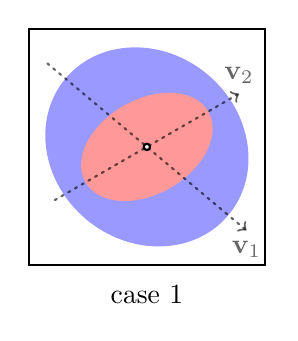
\begin{tikzpicture}[scale=1.5,thick,line cap=round]
	\tikzstyle{jiao}=[solid,circle,draw,fill=white,inner sep=.8pt];
	\draw[draw=none,rotate=50,fill=blue!40] (0,0) ellipse (0.8cm and 0.9cm);
	\draw[draw=none,rotate=30,fill=red!40]  (0,0) ellipse (0.6cm and 0.4cm);
	\draw[dotted,->,opacity=0.6] (140:1.1) -- (-40:1.1) node[below]{$\mathbf{v}_1$};
	\draw[dotted,->,opacity=0.6] (210:0.9) -- (30:0.9)  node[above]{$\mathbf{v}_2$};
	\draw (-1,-1) rectangle (1,1);
	\node[jiao] at (0,0) {};
	\node[label=below:{case 1}] at (0,-1) {};
\end{tikzpicture}

\end{document}
